%!TEX program = xelatex

\documentclass[compress]{beamer}
%--------------------------------------------------------------------------
% Common packages
%--------------------------------------------------------------------------

\definecolor{links}{HTML}{663000}
\hypersetup{colorlinks,linkcolor=,urlcolor=links}

\usepackage[english]{babel}
\usepackage{pgfpages} % required for notes on second screen
\usepackage{graphicx}

\usepackage{multicol}

\usepackage{tabularx,ragged2e}
\usepackage{booktabs}

\setlength{\emergencystretch}{3em}  % prevent overfull lines

\usetheme{hri}
\usetikzlibrary{shapes.geometric}
\usetikzlibrary{svg.path, matrix}
\usetikzlibrary{fpu,calc,fit,mindmap,backgrounds,positioning}

\usepackage{pgfplots}
\usepackage{pgfplotstable}
%\usepgfplotslibrary{external}
%\tikzexternalize 

\pgfmathdeclarefunction{gauss}{2}{%
      \pgfmathparse{1/(#2*sqrt(2*pi))*exp(-((x-#1)^2)/(2*#2^2))}%
      }


% Display the navigation bullet even without subsections
\usepackage{remreset}% tiny package containing just the \@removefromreset command
\makeatletter
\@removefromreset{subsection}{section}
\makeatother
\setcounter{subsection}{1}

\makeatletter
\let\beamer@writeslidentry@miniframeson=\beamer@writeslidentry
\def\beamer@writeslidentry@miniframesoff{%
  \expandafter\beamer@ifempty\expandafter{\beamer@framestartpage}{}% does not happen normally
  {%else
    % removed \addtocontents commands
    \clearpage\beamer@notesactions%
  }
}
\newcommand*{\miniframeson}{\let\beamer@writeslidentry=\beamer@writeslidentry@miniframeson}
\newcommand*{\miniframesoff}{\let\beamer@writeslidentry=\beamer@writeslidentry@miniframesoff}
\makeatother



\newcommand{\source}[2]{{\tiny\it Source: \href{#1}{#2}}}

\usepackage{tikz}
\usetikzlibrary{mindmap,backgrounds,positioning,calc,patterns}

\graphicspath{{figs/}}

\title{Data Analysis for HRI}
\subtitle{~}
\date{}
\author{Séverin Lemaignan}
\institute{{\bf Bristol Robotics Lab}\\University of the West of England}

\begin{document}

\miniframesoff

\licenseframe{github.com/severin-lemaignan/lecture-hri-data-analysis}

\maketitle

\miniframeson


\begin{frame}{In this lecture}

\begin{itemize}
    \item<+-> Two questions to answer:
        \begin{itemize}
            \item<+-> Are my groups different?
            \item<+-> Does a specific variable explain the difference?
        \end{itemize}
    \item<+-> Hands-on data analysis with Python!
\end{itemize}

\end{frame}



%%%%%%%%%%%%%%%%%%%%%%%%%%%%%%%%%%%%%%%%%%%%%%%%%%%%%%%%%%%%%%%%%
%%%%%%%%%%%%%%%%%%%%%%%%%%%%%%%%%%%%%%%%%%%%%%%%%%%%%%%%%%%%%%%%%
%%%%%%%%%%%%%%%%%%%%%%%%%%%%%%%%%%%%%%%%%%%%%%%%%%%%%%%%%%%%%%%%%

\section{Are my two groups different?}

\begin{frame}{A dataset}

    \centering

    \pgfplotstabletypeset[assign column name/.style={
                            /pgfplots/table/column name={\textbf{#1}}
                          },
                          col sep=comma, 
                          string type]{code/dataset1.csv}
\end{frame}

\imageframe[scale=0.8]{code/fig1.pdf}
\imageframe[scale=0.8]{code/fig2.pdf}
\imageframe[scale=0.8]{code/fig3.pdf}

\begin{frame}{}

    Is there a difference?

    \begin{itemize}
        \item Is the distribution the same?
        \item How big the difference? $\rightarrow$ \textbf{effect size}
        \item Could chance explain that difference?
    \end{itemize}
\end{frame}

\begin{frame}{Is the distribution the same?}

    Data often (but not always!) follows a
    \href{http://en.wikipedia.org/wiki/Normal_distribution}{normal} (or
    Gaussian) distribution. Two parameters: \textbf{mean $\mu$ and variance $\sigma^2$}.

    \begin{center}
        \resizebox{0.8\linewidth}{!}{
            \begin{tikzpicture}
                \begin{axis}[
                        no markers, domain=-5:5, samples=200,
                    axis lines*=left,
                    every axis y label/.style={at=(current axis.above origin),anchor=south},
                    every axis x label/.style={at=(current axis.right of origin),anchor=west},
                    height=5cm, width=\linewidth,
                    xtick={-5,...,5}, ytick={0.0,0.1,...,1.0},
                    enlargelimits=false, clip=false, axis on top,
                    grid = major
                ]
                    \addplot [very thick,yellow!50!black] {gauss(0,2.24)};
                    \addlegendentry{\tiny$\mu=0, \sigma^2=5.0$};
                    \addplot [very thick,green!50!black] {gauss(-2,0.71)};
                    \addlegendentry{\tiny$\mu=-2, \sigma^2=0.5$};
                    \addplot [very thick,red!50!black] {gauss(0,1)};
                    \addlegendentry{\tiny$\mu=0, \sigma^2=1.0$};
                    \addplot [very thick,blue!50!black] {gauss(0,0.45)};
                    \addlegendentry{\tiny$\mu=0, \sigma^2=0.2$};

                \end{axis}

                \node at (7,1) {\bubblemark{gauss2}};
            \end{tikzpicture}
        }
    \end{center}

    \pause

    Many statistical tests only work if the underlying data follows a normal
    distribution -- so-called \textbf{parametric tests}.

    \emph{You need to check that your data is normally distributed first! (for
    instance, by plotting it)}

\end{frame}

\begin{frame}{Compare distributions (histograms, density)}


    \begin{center}
        \includegraphics<1>[width=0.8\linewidth]{code/distributions-control.pdf}
        \includegraphics<2>[width=0.8\linewidth]{code/distributions.pdf}

    \only<1>{Control group}
    \only<2>{Control + condition group $\rightarrow$ beware the bimodal
    distribution!}
    \end{center}

\end{frame}

\imageframe[scale=0.8, caption={Show the underlying data!}]{code/fig4.pdf}

\begin{frame}{Anscombe's quartet}
    \only<1>{
        \small
    \begin{tabular}{@{}llllllll@{}}
\toprule
\multicolumn{2}{l}{\textbf{I}} & \multicolumn{2}{l}{\textbf{II}} & \multicolumn{2}{l}{\textbf{III}} & \multicolumn{2}{l}{\textbf{IV}} \\ \midrule
\textit{x}     & \textit{y}    & \textit{x}     & \textit{y}     & \textit{x}      & \textit{y}     & \textit{x}     & \textit{y}     \\ \midrule
10.0           & 8.04          & 10.0           & 9.14           & 10.0            & 7.46           & 8.0            & 6.58           \\
8.0            & 6.95          & 8.0            & 8.14           & 8.0             & 6.77           & 8.0            & 5.76           \\
13.0           & 7.58          & 13.0           & 8.74           & 13.0            & 12.74          & 8.0            & 7.71           \\
9.0            & 8.81          & 9.0            & 8.77           & 9.0             & 7.11           & 8.0            & 8.84           \\
11.0           & 8.33          & 11.0           & 9.26           & 11.0            & 7.81           & 8.0            & 8.47           \\
14.0           & 9.96          & 14.0           & 8.10           & 14.0            & 8.84           & 8.0            & 7.04           \\
6.0            & 7.24          & 6.0            & 6.13           & 6.0             & 6.08           & 8.0            & 5.25           \\
4.0            & 4.26          & 4.0            & 3.10           & 4.0             & 5.39           & 19.0           & 12.50          \\
12.0           & 10.84         & 12.0           & 9.13           & 12.0            & 8.15           & 8.0            & 5.56           \\
7.0            & 4.82          & 7.0            & 7.26           & 7.0             & 6.42           & 8.0            & 7.91           \\
5.0            & 5.68          & 5.0            & 4.74           & 5.0             & 5.73           & 8.0            & 6.89           \\ \bottomrule
\end{tabular}
}
    \only<2>{
    \begin{center}
        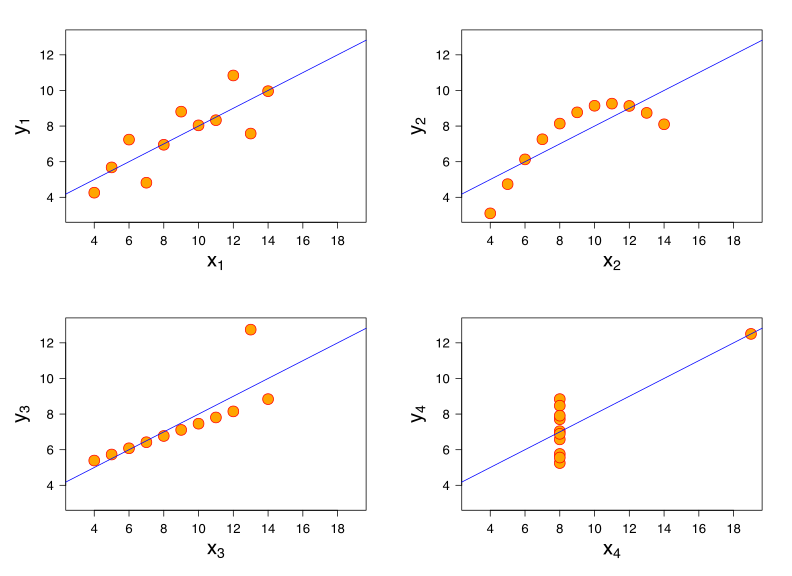
\includegraphics[width=0.8\linewidth]{Anscombe's_quartet}
    \end{center}
}
\end{frame}


\begin{frame}{Alternative dataset}

    \begin{columns}
        \begin{column}{0.5\linewidth}

            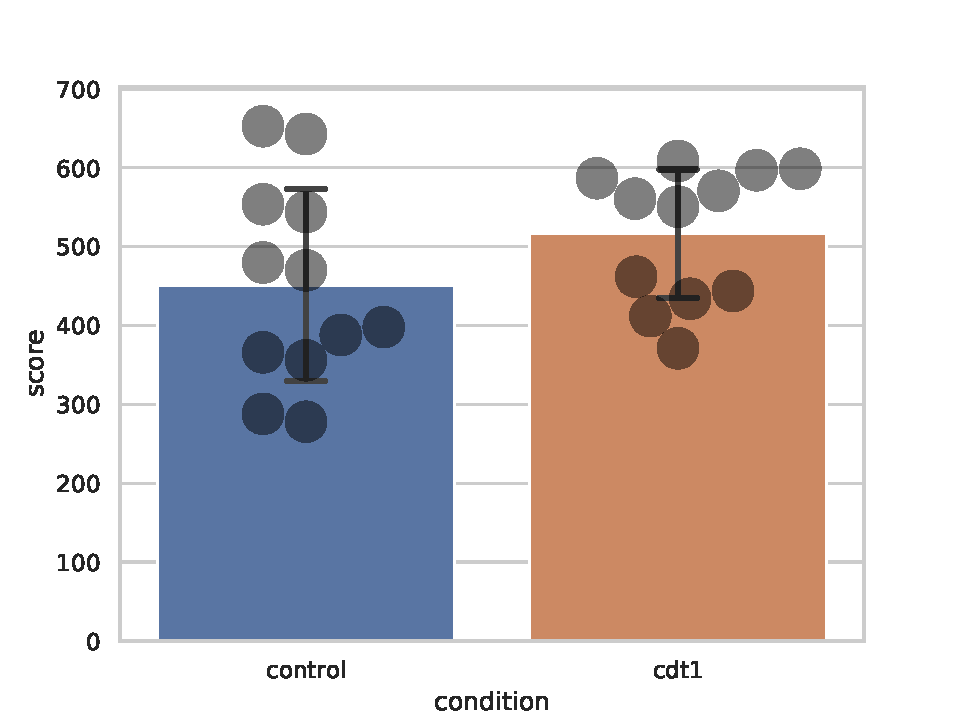
\includegraphics[width=\columnwidth]{code/dataset2-cdts.pdf}
        \end{column}
        \begin{column}{0.5\linewidth}
            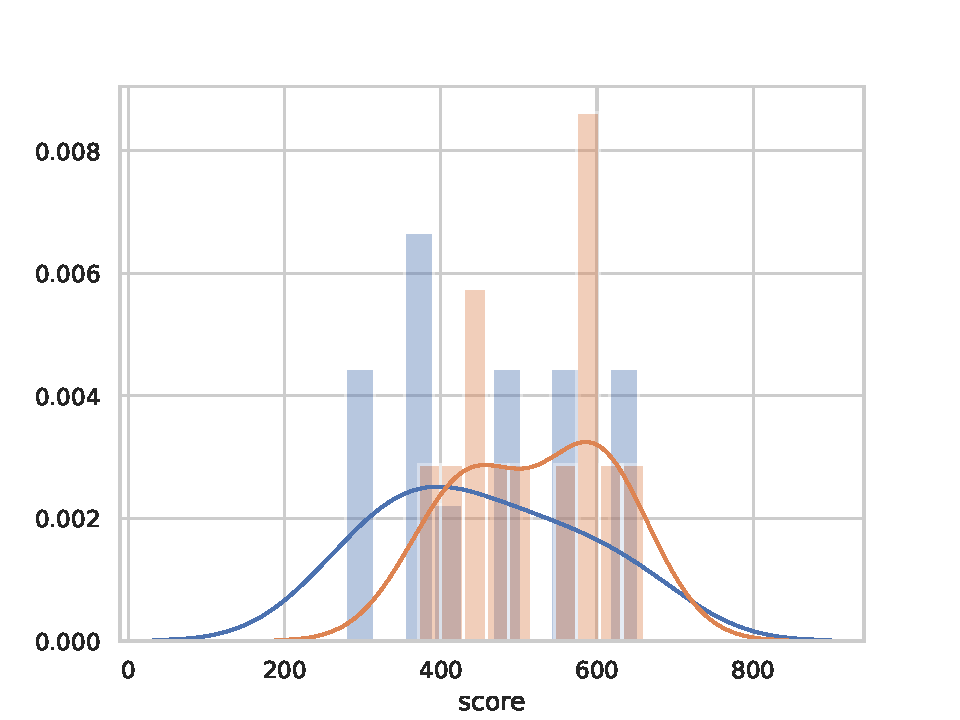
\includegraphics[width=\columnwidth]{code/distributions2.pdf}

        \end{column}
    \end{columns}

    \begin{center}
        \begin{tabular}{lrrrrrrrr}
            \toprule
            {} &  mean &         std\\ \midrule
            cdt1      &   516.5 & 85.3 \\
            control   &   451.5 & 127.1\\
            \bottomrule
        \end{tabular}
    \end{center}

\end{frame}


\begin{frame}{How big is the difference?}


\end{frame}

\begin{frame}{Difference due to chance?}

    [impact of n on p]
\end{frame}


\begin{frame}{Be careful with "Statistically Significant"!}

    [low p value, but low effect size]
\end{frame}

\begin{frame}{Statistical power analysis}
\end{frame}

\section{Does one variable explain the difference?}

\begin{frame}{Correlation is not causation}
\end{frame}

\begin{frame}{Effect size}
    Quantify the degree of association between two related variables.
\end{frame}


\section{In practice}



\begin{frame}{The tools}

    Data analysis tools:

    \begin{itemize}
        \item R: \url{www.r-project.org}
        \item Python's Pandas: \url{pandas.pydata.org}
    \end{itemize}

    \pause

    Jupyter notebooks are a  great way of creating an interactive, easy-to-follow,
    data analysis.

\end{frame}

\begin{frame}{(side note on Python for data analysis)}

    Python is the leading language in data analysis/data mining/machine
    learning. \textbf{Learn it!}

    \pause

    Large set of tools $\Rightarrow$ the SciPy landscape can be confusing at first:

    \pause

    \begin{itemize}
        \item<+-> \texttt{numpy}, \texttt{scipy}: the 'math' core
        \item<+-> \texttt{ipython}, \texttt{Jupyter notebook}: interactive Python
        \item<+-> \texttt{matplotlib}, \texttt{seaborn}: data visualisation
            (including plotting)
        \item<+-> \texttt{pandas}, \texttt{statsmodels}: stats, data analysis (modelled after R)
        \item<+-> \texttt{scikit-learn} (along with specialist ML libraries:
            \textsc{TensorFlow}, \textsc{pyTorch}): machine learning
        \item<+-> \texttt{anaconda} (and a few other): Python distribution for
            scientific computing
    \end{itemize}

\end{frame}

\begin{frame}[plain]
    \Large
    \bf
    \centering
    Let's give it a go!
\end{frame}

\end{document}
